\documentclass[conference,harvard,brazil,english]{sbatex}
\usepackage[T1]{fontenc}
\usepackage[utf8]{inputenc}
\usepackage{ae}
\usepackage{graphicx}
%
% LaTeX2e class SBATeX
%
% Versão 1.0 alpha
%   Walter Fetter Lages
%   w.fetter@ieee.org
%
% Este arquivo cba.tex é uma adaptação do arquivo revista.tex,
% Versão: 1.0 alpha, desenvolvido por Maurício C. de Oliveira,
% mcdeoliveira@ieee.org.
%
% As adaptações fazem com que, por default, sejam utilizadas
% as opções adequadas para o formato do CBA ou SBAI, ao contrário do arquivo
% revista.tex, que, por default, utiliza opções adequadas para o formato
% da Revista da SBA.
%
%
% --------------------------------------------------
%
% Para compilar este exemplo use a seqüência de comandos:
%
%     latex cba
%     bibtex cba
%     latex cba
%     latex cba
%
% Para gerar um arquivo Postscript (.ps):
%
%     dvips -t a4 cba
%
% Para gerar um arquivo Portable Document Format (.pdf):
%
%     dvips -Ppdf -t a4 cba
%     ps2pdf -dMaxSubsetPct=100 -dSubsetFonts=true -dEmbedAllFonts=true -dCompatibilityLevel=1.2 -sPAPERSIZE=a4 cba.ps
%

% --------------------------------------------------
%  Estes comandos são necessários apenas para a
%  a geração deste artigo exemplo. Eles não fazem
%  parte do estilo SBATeX.
% --------------------------------------------------
\makeatletter
\def\verbatim@font{\normalfont\ttfamily\footnotesize}
\makeatother
\usepackage{amsmath}
% --------------------------------------------------


\begin{document}

% CABEÇALHO

\title{Comparação entre o método dos Mínimos Quadrados e Maximização da Correntropia do Erro aplicados ao Controle Adaptativo}

%%%%%%%%%%%%%%%%%%%%%%%%%%%%%%%%%%%%%%%%%%%%%%%%%%%%%%%%%%%%%
%
% O processo de revisao do CBA 2014 sera DOUBLE BLIND, portanto NAO inclua
% autores na versão que será submetida para revisão
%
%%%%%%%%%%%%%%%%%%%%%%%%%%%%%%%%%%%%%%%%%%%%%%%%%%%%%%%%%%%%%

\author{~}{~}
\address{~~\\ ~~\\ ~~}

\twocolumn[

\maketitle

\selectlanguage{english}
\begin{abstract}
  The continuous-time recursive least squares with forgetting factor algorithm as a means of estimating the unknown parameters of a linear system has been a mainstay of the Adaptive Control field for more than 20 years. The use of the square error as a cost function that must be minimized(MSE) with respect to certain parameters is well known in the literature and produces good results in a variety o applications. Mathematically, it has good properties when the uncertainty in the data has a gaussian-like distribution. However, researches in the field of Information Theory have, for some time now, been presenting descriptors in a framework called Information Theoretic Learning(ITL) that better characterize data when the uncertainty is non-gaussian in some sense. This is certainly true in a variety of applications of Adaptive Control, where the controller must deal with change over time in plant parameters and different operating conditions. Noise and input perturbation can come in a variety of forms, and although some of them are indeed gaussian-like, most are not.  
  
  The aim of this paper is to present an algorithm that translates the Maximum Correntropy concept to estimate online the unknown parameters of an LIT System, as opposed to Minimum Square Error estimation.   
      
\end{abstract}

\keywords{Adaptive Control, Estimation, Information Theory, Information Theoretic Learning, Maximização da Correntropia}

\selectlanguage{brazil}
\begin{abstract}
  
  O uso do algoritmo de mínimos quadrados de tempo contínuo recursivo com fator de esquecimento como uma forma de estimar os parâmetros desconhecidos de um sistema linear tem sido uma ferramenta importante no campo do Controle Adaptativo por mais de 20 anos. O uso do erro quadrado como uma função de custo que precisa ser minimizada com respeito a um conjunto de parâmetros é bem conhecida na literatura e apresenta bons resultados numa variedade de aplicações. Matematicamente, tem boas propriedades quando a incerteza nos dados possui uma distribuição gaussiana. No entanto, pesquisadores no campo da Teoria da Informação têm apresentado descritores que melhor caracterizam os dados quando a incerteza tem distribuição não-gaussiana em algum sentido. Isto é certamente verdade em muitas aplicações de Controle Adaptativo, once o controlador precisa lidar com a mudança ao longo do tempo nos parâmetros planta e com condições de operações diferentes. Ruído e perturbação de entrada podem ser encontrados em uma variedade de formas, e apesar de algumas delas serem gaussianas, a maioria não o é.
  
  O objetivo deste trabalho é apresentar um algoritmo que traduza o conceito de Maximização da Correntropia para estimar em tempo real os parâmetros desconhecidos de um sistema LIT, e comparar estes resultados com os obtidos pelo algoritmo que minimiza o erro quadrado.
  
  
  
\end{abstract}

\keywords{Controle Adaptativo, Estimação, Teoria da Informação, Minimização de Entropia da Informação}
]

% CONTRIBUIÇÃO

\selectlanguage{brazil}

\section{Introdução}

O controle adaptativo é uma alternativa popular quando é necessário lidar com plantas lineares que apresentam incerteza paramétrica ou variação temporal lenta nos valores dos parâmetros. O método indireto, no qual, dados os sinais de entrada e saída disponíveis para medição, um estimador de mínimos quadrados apresenta valores das estimativas dos parâmetros da planta que são usadas para atualizar os parâmetros do controlador, apresenta resultados satisfatórios e a literatura disponível é extensiva. A formulação matemática usada para implementar um método de mínimos quadrados recursivo em tempo contínuo se presta facilmente à solução do problema simultâneo da estimação e controle de uma planta linear de grau relativo qualquer. Embora a implementação seja abordada de forma determinística na literatura de controle adaptativo, suas propriedades  em relação à ruídos gaussianos estão bem caracterizadas.\\  

Nos últimos 25 anos, pesquisadores na área de teoria da informação tem proposto um ferramental conhecido com Aprendizado por Teoria da Informação \cite{principebook}, onde descritores estatísticos tradicionais tais como variância e correlação são substituídos por entropia e correntropia por exemplo. Estes conceitos se estendem naturalmente ao problema da otimização de uma função de custo com relação a um conjunto de parâmetros. Como a correntropia é sensível aos momentos de ordem superior a dois na distribuição dos dados, um algoritmo que minimiza a entropia do erro poderá tratar de uma classe maior de ruídos de forma estável. Neste trabalho propomos uma estratégia de Controle Adaptativo Indireto usando um Estimador de Maximização da Correntropia do Erro.


\section{Preliminares Matemáticas}

Discutimos aqui algumas ideias referentes ao controle adaptativo quando o objetivo é fazer com que a planta rastreie a saída de um modelo de referência. Consideramos que apenas a entrada $u(t)$ e a saída $y(t)$ estão disponíveis para medição.

\subsection*{A. Estimador Via Mínimos Quadrados com Fator de Esquecimento}

Seja a planta linear invariante no tempo, controlável e observável descrita por sua função de transferência:
\begin{equation}
G_p(s) = \frac{N_p(s)}{D_p(s)} = \frac{b_0 + b_1 s + ... + b_{n-1} s^{n-1}}{a_0 + a_1 s+ ... + a_n s^n}
\end{equation}

Onde usamos $a_n = 1$ sem perda de generalidade. E seja o vetor de parâmetros da planta a ser estimado:
\begin{equation*}
\theta^* = [b_{n-1}, b_{n-2}, ...~ , b_1, b_0, a_{n-1}, a_{n-2}, ...~ , a_1, a_0]^T
\end{equation*}

E portanto a planta pode ser parametrizada da seguinte forma:

\begin{equation}
y = {\theta^*}^T Y
\end{equation}

Onde:

\begin{equation*}
Y = [u^{(n-1)},u^{(n-2)},...,u,-y^{(n-1)},-y^{(n-2)},-y]
\end{equation*}

É necessário construir um estimador para os $2n$ parâmetros da planta. Como apenas $u(t)$ e $y(t)$ estão disponíveis para medição e não é desejável trabalhar com derivadas dos sinais, criamos os sinais adicionais necessários através de filtros. Tal que, seja um filtro estável $\Lambda(s)$:

\begin{equation}
\Lambda(s) = s^n + \lambda_{n-1} s^{n-1} + ... + \lambda_0
\end{equation}

E seja:

\[ \lambda^T = \begin{bmatrix}
            \lambda_{n-1}, & \lambda_{n-2}, & ..., & \lambda_0
          \end{bmatrix}
\]

Podemos expressar:

\begin{equation}
\Lambda(s) = s^n + \lambda^T\alpha_{n-1}
\end{equation}

Sendo:

\begin{equation*}
\alpha_{n-1} = [s^{(n-1)},s^{(n-2)},...,s^0]^T
\end{equation*}

A partir de $y(t)$, criamos um sinal $z(t)$: 

\begin{equation}
\begin{array}{l}
z = \frac{s^n y}{\Lambda(s)} \\
= \frac{\Lambda(s) - \lambda^T\alpha_{n-1}(s)}{\Lambda(s)}y = y - \lambda^T\alpha_{n-1}(s)
\end{array}
\end{equation}

e calculamos:

\begin{equation}
\phi_1 = \frac{\alpha_{n-1}(s)}{\Lambda(s)} u
\end{equation}

\begin{equation}
\phi_2 = -\frac{\alpha_{n-1}(s)}{\Lambda(s)} y
\end{equation}

Desta forma:

\begin{equation}
z = {\theta^*}^T \phi
\end{equation}

E resta apenas estimar $\theta^*$ a partir do sinal $z$ e do regressor $\phi = [\phi_1, \phi_2]^T$, podemos também expressar essa parametrização de forma compacta, em espaço de estados: 

\begin{equation}
\label{eq:sigmaIDMARC}
\displaystyle 
\begin{array}{l}

        \dot{\phi}_1(t) = \Lambda_c \phi_1 + lu       \\
        \dot{\phi}_2(t) = \Lambda_c \phi_2 + ly       \\
        y = \theta^*_\lambda \phi                     \\
        z = y + \lambda^T\phi_2 = {\theta^*}^T \phi  
         
\end{array}
\end{equation}

Em que:

\begin{equation*}
\theta^*_\lambda = [{\theta_1^*}^T, {\theta_2^*}^T - \lambda^T]^T
\end{equation*}

Onde o par  $\{ \Lambda_c, l \}$ representa um filtro estável de ordem $n-1$, e $\Lambda(s)$ associado ao par é mônico e Hurwitz . $\phi$ o vetor de sinais concatenado a partir de $\phi_1$ e $\phi_2$. Seja então a estimativa $\hat{z}$ de $z$ o erro de estimação normalizado $\epsilon$:

\begin{equation}
\displaystyle 
\begin{array}{l}

        \hat{z} = \theta^T \phi \\
        \epsilon = \frac{z - \hat{z}}{m^2}
         
\end{array}
\end{equation}

Onde $m = 1+n_s^2$ tal que $\phi/m \in \mathcal{L}_\infty$. A função de custo:

\begin{equation}
\displaystyle 
\begin{array}{r}

       J(\theta) = \frac{1}{2} \int_{0}^{t} e^{-\beta(t - \tau)} \frac{[z(\tau) - \theta^T(t)\phi(\tau)]}{m^2(\tau)} d\tau \\
        + \frac{1}{2} e^{-\beta t}(\theta - \theta_0)^TQ_0(\theta - \theta_0)
         
\end{array}
\end{equation}

Tem gradiente da forma:

\begin{equation}
\begin{array}{r}
\nabla J(\theta) = e^{-\beta t}Q_0 (\theta(t)-\theta_0) - \\
                    -\int_{0}^t e^{-\beta(t - \tau)} \frac{[z(\tau) - \theta^T(t)\phi(\tau)]}{m^2(\tau)}\phi(\tau) d\tau
\end{array}
\end{equation}

E igualando a 0 se obtém:

\begin{equation}
\begin{array}{l}
\theta(t) = P(t)[e^{-\beta t}Q_0 \theta_0 -\\
                 \int_{0}^t e^{-\beta(t - \tau)}\frac{[z(\tau)\phi(\tau)]}{m^2(\tau)} d\tau]         
\end{array}
\end{equation}

Com:

\begin{equation}
P^{-1} = [e^{-\beta t}Q_0 - \int_{0}^t e^{-\beta(t - \tau)}\frac{[\phi(\tau)\phi^T(\tau)]}{m^2(\tau)} d\tau]   
\end{equation}

Como $\phi\phi^T$ é semi definida positiva a cada instante e $Q_0 = Q_0^T >0$ então $\exists P(t), \forall t$. Fazendo uso da identidade:

\begin{equation}
\frac{d PP^{-1}}{dt} = \dot{P}P^{-1} + P\frac{d P^{-1}}{dt} = 0
\end{equation}

Podemos mostrar que $\dot{P}$ satisfaz a equação diferencial:

\begin{equation}
 \dot{P} = \beta P - P\frac{\phi \phi^T}{m^2}P
\end{equation}

Desta forma, o cálculo da inversa é evitado gerando P como a solução de uma equação diferencial. Usando o mesmo raciocínio para $\theta(t)$ e diferenciando em relação ao tempo usando o resultado obtido para P diretamente e $\epsilon m^2 = z- \theta^T \phi$, podemos obter:

\begin{equation}
\dot{\theta} = P\epsilon \phi
\end{equation}

Que garante estimativa limitada e convergência para o valor correto $\theta^*$ desde que os sinais de entrada sejam limitados e o sinal de referência $\phi$ seja Persistentemente Excitante(PE). Este algoritmo é chamado de \emph{continuous-time recursive least squares algorithm with forgetting factor} e as provas de estabilidade e a derivação usadas podem ser encontradas em \cite{ioannou2}.

\subsection*{B. Posicionamento de Polos}

Sabemos, pelo princípio do modelo interno, que para que uma planta seja capaz de rastrear um determinado sinal ou rejeitar uma perturbação, é necessário que a estrutura da planta em malha direta contenha um polo capaz de gerar aquele sinal ou perturbação. De tal forma que, no design do controlador, se faz necessário introduzir um polinômio $Q_m(s)$ no denominador tal que a estrutura do controlador se torna:
\begin{equation}
C(s) = \frac{P(s)}{L(s)Q_m(s)}
\end{equation}

Usando uma malha de realimentação unitária, chegamos a uma função de transferência tal que:

\begin{equation}
G_{mf}(s) = \frac{P(s)N_p(s)}{L(s)Q_m(s)D_p(s) + N_p(s)P(s)}
\end{equation}

Uma estratégia explorada na literatura \cite{chen,ogata} para garantir a estabilidade do controlador e o objetivo de rastreamento e rejeição da perturbação é a de escolher um polinômio $A^*(s)$ e resolver a equação diofantina da forma:

\begin{equation}
L(s)Q_m(s)D_p(s) + N_p(s)P(s) = A^*(s)
\end{equation}

Com relação aos polinômios do numerador e denominador do controlador $C(s)$,que são $P(s)$ e $L(s)$, de forma que os polos da função de transferência em malha fechada correspondam aos polos de $A^*(s)$. Esta estratégia é conhecida como \emph{Controle por Posicionamento de Polos}.

Porém desejamos realizar simultaneamente a estimação e controle. Desta forma escolhemos como estratégia de controle o posicionamento adaptativo de polos, que é predicado na resolução da mesma equação diofantina para o polinômio desejado $A^*$ a cada iteração da simulação, com base nas estimativas dos polinômios do numerador e denominador da planta $\hat{N}_p(s)$ e $\hat{D}_p(s)$:

\begin{equation}
\hat{L} Q_m \hat{D}_p + \hat{P} \hat{N}_p = A^*
\end{equation}

Fazendo $D(s) = \hat{D}_p(s) Q_m(s)$ e $N(s) = N_p(s)$ a equação é resolvida através da montagem da matriz de Sylvester, tal que:\\



\[ S_m = \begin{bmatrix}
D_0 & D_1 & ... & D_n     & 0   & ... & 0  \\
N_0 & N_1 & ... & N_n     & 0   & ... & 0  \\
0   & D_0 & ... & D_{n-1} & D_n & ... & 0  \\
0   & N_0 & ... & N_{n-1} & N_n & ... & 0  \\
... & ... & ... & ...     & ... & ... & ...\\
0   & 0   & ... & 0       & D_0 & ... & D_n\\
0   & 0   & ... & 0       & N_0 & ... & N_n
\end{bmatrix}
\]

Onde $D_0,...,D_n$ e $N_0,...,N_n$ são os coeficientes dos polinômios D(s) e N(s) respectivamente.

\[
 v = \begin{bmatrix}
     L_0 & P_0 & L_1 & P_1& ... & L_m & P_m
     \end{bmatrix}
\]

Onde $L_0,...,L_m(s)$ e $P_0,...,P_m$ são os coeficientes dos polinômios L(s) e P(s) respectivamente.

\[
 f = \begin{bmatrix}
     F_0 & F_1 & ... & F_n & F_{n+1} & ... & F_{n+m}
 \end{bmatrix}
\]

Onde $F_0,...,F_{n+m}$ são os coeficientes do polinômio $A^*(s)$ escolhido. De tal forma que

\begin{equation}
S_m^T v^T = f^T
\end{equation}

E resovendo para $v$ obtemos a função de transferência $C(s)$ do controlador.\\

Tal que o sinal de controle realimentado é:\\

\begin{equation}
u_p = (\Lambda - \hat{L} Q_m)\frac{1}{\Lambda} u_p - \hat{P} \frac{1}{\Lambda}(y_p - r)
\end{equation}

Onde $\Lambda(s)$ representa um polinômio com autovalores no semiplano esquerdo escolhido arbitrariamente. A medida que as estimativas $\hat{N}_p$ e $\hat{D}_p$ convergem, os parâmetros do controlador são atualizados e a função de transferência em malha fechada se aproxima de $A^*(s)$. A prova de estabilidade deste método está disponível na literatura da área de controle adaptativo. \cite{ioannou2}\cite{krstic}\cite{tao} \\
\section{Estimador através da Maximização da Correntropia do Erro}

Do ferramental disponível para Aprendizado a partir da Teoria da Informação, apresentamos a seguinte figura:\\

\begin{figure}[htpb!]
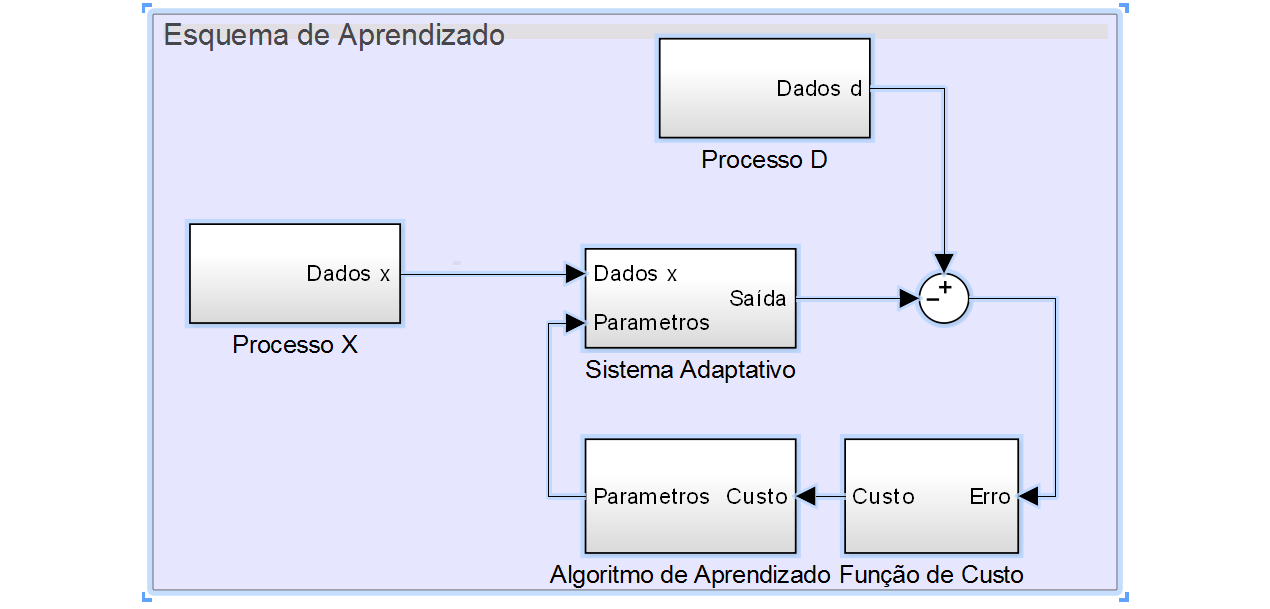
\includegraphics[width = \linewidth]{./pics/ITL_Esquema.png}
\caption{Sistema Adaptativo Genérico descrito no ferramental ITL}
\end{figure}

De forma que parece existir uma equivalência com o controle adaptativo:\\

\begin{figure}[htpb!]
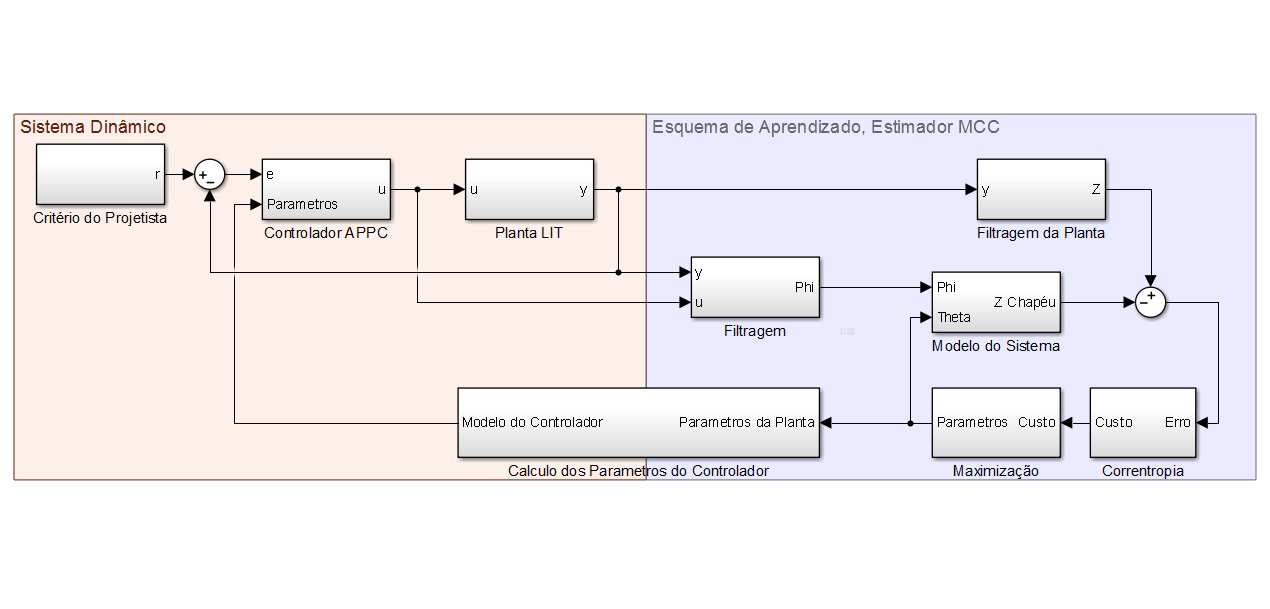
\includegraphics[width = \linewidth]{./pics/ITL_Controle_Adaptativo.png}
\caption{Controle Adaptativo Indireto usando um estimador de parâmetros baseado em Maximização da Correntropia do Erro}
\end{figure}

Assumindo que a medição de $y(t)$ esteja contaminada por algum tipo de ruído, seu filtrado $z(t)$ se torna um processo estocástico, assim como a estimativa $\hat{z}(t)$. Seja então a Correntropia \cite{principe1} \cite{chen2} entre as variáveis aleatórias $Z$ e $\hat{Z}$:

\begin{equation}
V(Z,\hat{Z}) = \mathbf{E}(k_\sigma(Z-\hat{Z}))
\end{equation}

Um estimador por amostras da correntropia entre estas variáveis aleatórias pode ser escrito como:

\begin{equation}
\hat{V}_{N,\sigma}(Z,\hat
{Z})  = \frac{1}{N}\sum_{i=1}^N k_{\sigma} (z_i - \hat{z}_i)
\end{equation}

Onde $z_i$ e $\hat{z}_i$ são amostras colhidas sequencialmente a partir das realizações $z(t)$ e $\hat{z}(t)$. Desta forma, se escolhermos $N$ amostras dos sinais $z_i$ e $\phi_i$, podemos expressar:

\begin{equation}
\hat{V}_{N,\sigma}(Z,\hat
{Z})  = \frac{1}{N}\sum_{i=1}^N k_{\sigma} (z_i - \theta^T(t)\phi_i)
\end{equation}

Cujo gradiente em relação aos parâmetros $\theta$, com kernel gaussiano é:

\begin{equation}
\nabla\hat{V}_{N,\sigma}(\theta) = \frac{1}{\sqrt{2\pi}\sigma^3 N}\sum_{i=1}^N \frac{-(z_i - \theta^T \phi_i)}{m^2}(-\phi_i) e^{-\frac{(z_i - \theta^T(t)\phi_i)^2}{2 \sigma^2 m^2}}
\end{equation}

É possível escolher este estimador da correntropia de forma que a cada passo da simulação uma amostra seja colhida e maximizar seu valor de saída ajustando o valor dos parâmetros $\theta$ e reavaliando o valor de $\hat{z}_i$ a cada iteração. Assim, cada amostra escolhida implica no aumento do custo computacional do algoritmo. No entanto, a depender do intervalo entre a colheita das amostras, dentre outros fatores, o aumento do custo computacional pode não se traduzir diretamente em uma melhoria do processo de estimação. Por exemplo, se duas amostras forem colhidas em instantes de tempo $t_i$ e $t_j$ com intervalo muito pequeno, é provável que os vetores $\phi_i$ e $\phi_j$ associados sejam praticamente ou numericamente LD entre si, de forma que carreguem informações iguais sobre a direção e sentido do máximo do estimador da correntropia. De fato, a escolha de amostras relevantes para o estimador da correntropia não é um problema trivial.\\  

Com base nestes conceitos escolhemos como função de custo a correntropia com $N=1$, isto é, considerando apenas a amostra mais recente do erro $\epsilon$ com kernel gaussiano entre o filtrado da saída da planta e sua estimativa:\\

\begin{equation}
 \displaystyle 
 \begin{array}{l}
 J(\theta) =\frac{1}{\sqrt{2\pi}\sigma} e^{-\epsilon^2/2\sigma^2} =\frac{1}{\sqrt{2\pi}\sigma} e^{-\frac{(z - \theta^T \phi)^2}{2 m^2 \sigma^2}}\\
 \nabla J(\theta) = \epsilon \phi \frac{1}{\sqrt{2\pi}\sigma^3} e^{-\frac{\epsilon^2}{2 \sigma^2}}        
 \end{array}
\end{equation}

Esta formulação é similar ao gradiente estocástico(SGD) na sua forma mais simples, que pode ser encontrado por exemplo em \cite{Bottou2010}. Porém, ao contrário do algoritmo SGD, não dispomos de um estudo detalhado de suas propriedades de convergência na presença do ruído. Esperamos, como no argumento usado para o SGD, que a função de custo $J(\theta)$ produzida a partir do estimador se comporte como o valor esperado em (24), que corresponde à correntropia entre as variáveis $Z$ e $\hat{Z}$.\\

Esta escolha de estimador para a correntropia permite gasto computacional baixo, já que não é preciso armazenar múltiplas amostras do erro $\epsilon(t)$ e do regressor $\phi(t)$, o que se presta ao objetivo de realizar a estimação e controle simultâneamente.\\

Caminhando na direção do gradiente de forma a maximizar a função de custo, uma escolha possível de lei adaptativa é:

\begin{equation}
\dot{\theta} = \Gamma \nabla J(\theta)
\end{equation}

Onde $\Gamma \in \mathcal{R}^{2n\times2n}$, $\Gamma = \Gamma^T > 0$ é uma matriz de ganhos adaptativos de forma a ajustar a velocidade da convergência dos parâmetros $\theta$. De forma que temos a seguinte lei adaptativa para os parâmetros $\theta$:

\begin{equation}
\displaystyle 
\begin{array}{l}
\dot{\theta} = \Gamma \nabla J(\theta) = \Gamma \epsilon \phi \frac{1}{\sqrt{2\pi}\sigma^3} e^{-\frac{\epsilon^2}{2\sigma^2}}\\
\end{array}
\end{equation}

Caracterizamos o erro paramétrico de estimação:

\begin{equation}
\tilde{\theta} = \theta - \theta^*
\end{equation}

Para analise da estabilidade desta lei adaptativa, e fazendo uso do erro paramétrico $\tilde{\theta}$, propomos a seguinte candidadata:

\begin{equation}
V(\tilde{\theta}) = \tilde{\theta}^T \Gamma^{-1} \tilde{\theta}>0
\end{equation}

Obtendo sua derivada $\dot{V}(\tilde{\theta})$ e substituindo $\dot{\tilde{\theta}}$ (pois consideramos uma planta LIT) por $\dot{\theta}$ chegamos a:

\begin{equation}
\dot{V}(\tilde{\theta}) = -2\tilde{\theta}^T \phi \epsilon \frac{1}{\sqrt{2\pi}\sigma^3}e^{-\frac{\epsilon^2}{2\sigma^2}}
\end{equation}

E finalmente, substituindo $\tilde{\theta}^T\phi$ por $\epsilon m^2$ 

\begin{equation}
\displaystyle 
\dot{V}(\tilde{\theta}) = -\frac{\epsilon^2 m^2}{\sqrt{2\pi}\sigma^3}e^{-\frac{\epsilon^2}{2\sigma^2}} \leq 0
\end{equation}

Que é semi definida negativa e implica, juntamente com as propriedades dos sinais envolvidos na estimação, em:\\
\flushleft
(i) $\epsilon, \epsilon n_s, \theta, \dot{\theta} \in \mathcal{L}_\infty$\\
(ii)$ \epsilon, \epsilon n_s, \dot{\theta} \in \mathcal{L}_2$\\
(iii) se $n_s, \phi \in \mathcal{L}_\infty$ e adicionalmente $\phi$ PE então $\theta(t)$ converge assintoticamente para $\theta^*$


\section{Simulações}



Realizamos simulações comparativas entre o controlador APPC com estimador usando critério LSE de tempo contínuo e o mesmo controlador com estimador usando o critério de maximização da correntropia (MCC) discutido. Os parâmetros de simulação foram escolhidos da seguinte forma:
\begin{equation}
\label{eq:Distribuição do ruído}
\displaystyle 
\begin{array}{l}
       N_p(s)          = 0.2s+2\\
       D_p(s)          = s^2+3s+4\\
       A^*(s)          = s^4+5.2s^3+12.4s^2+12.6s+6\\
       \hat{N}_{p0}(s) = 0.1s+3  \\
       \hat{D}_{p0}(s) = s^2+2s+5\\
       Qm(s)           = s       \\ 
       \Lambda(s)      = s^2+4s+5\\
       \Gamma = P_0 = 100I \\
       \sigma = 1
\end{array}
\end{equation}
%editar as figuras, revisar os valores de simulação % feito.
Com a planta partindo do repouso. 

\subsection{Sem ruído}

Os resultados se encontram nas Figuras 3 e 4, para o LSE e MCC respectivamente.

\begin{figure}[htpb!]
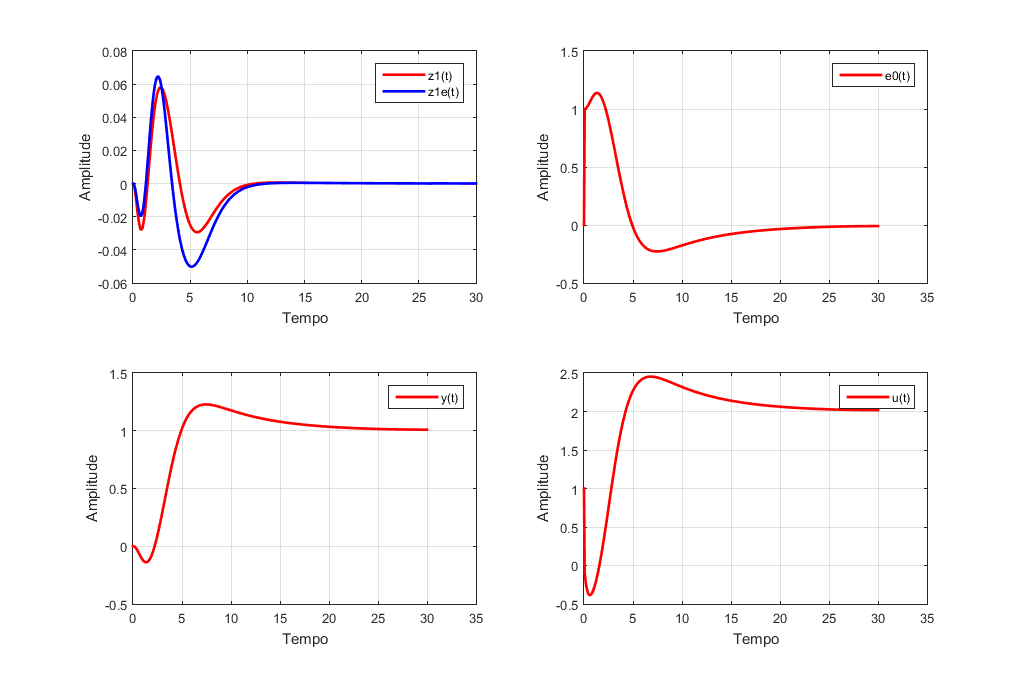
\includegraphics[width = \linewidth]{./pics/APPC_MSE_Ideal.png}
\caption{APPC-LSE num ambiente de simulação sem ruído, observa-se a convergência de $\hat{z}$ para $z$ e portanto $\epsilon \rightarrow 0$ a medida que $t \rightarrow \infty$, como esperado }
\end{figure}

\begin{figure}[htpb!]
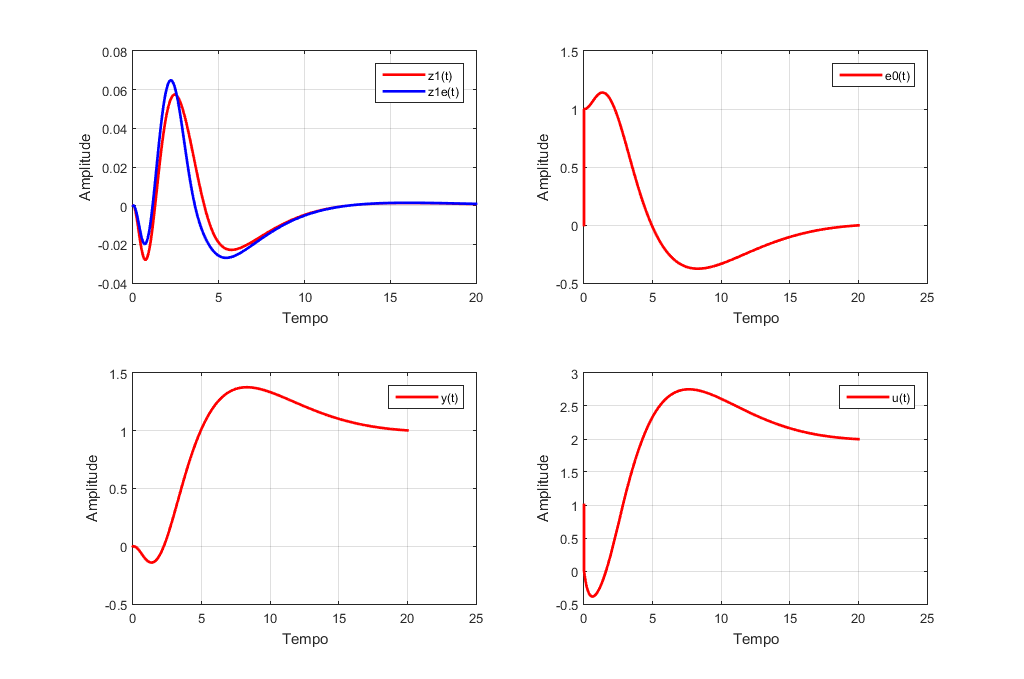
\includegraphics[width = \linewidth]{./pics/APPC_Correntropia_Ideal.png}
\caption{APPC-MCC num ambiente de simulação  sem ruído, similarmente ao APPC-LSE, observamos a convergência de $\epsilon$ para 0}
\end{figure}

\subsection{Com Ruído Gaussiano de média 0 e variância 0.05}


Os resultados se encontram nas Figuras 5 e 6, para o LSE e MCC respectivamente.

\begin{figure}[htpb!]
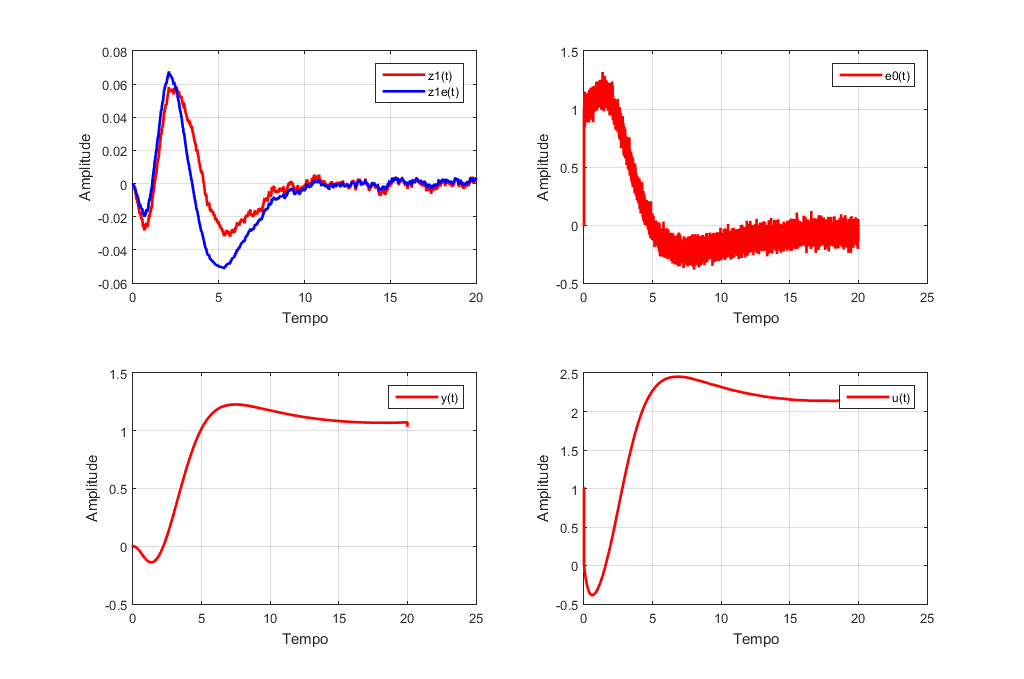
\includegraphics[width = \linewidth]{./pics/APPC_MSE_Ruido_Gaussiano.png}
\caption{APPC-LSE num ambiente de simulação com ruído gaussiano aditivo de média 0 e variância 0.05, observa-se a convergência de $\hat{z}$ para $z$ e portanto $\epsilon \rightarrow 0$ a medida que $t \rightarrow \infty$, como esperado }
\end{figure}

\begin{figure}[htpb!]
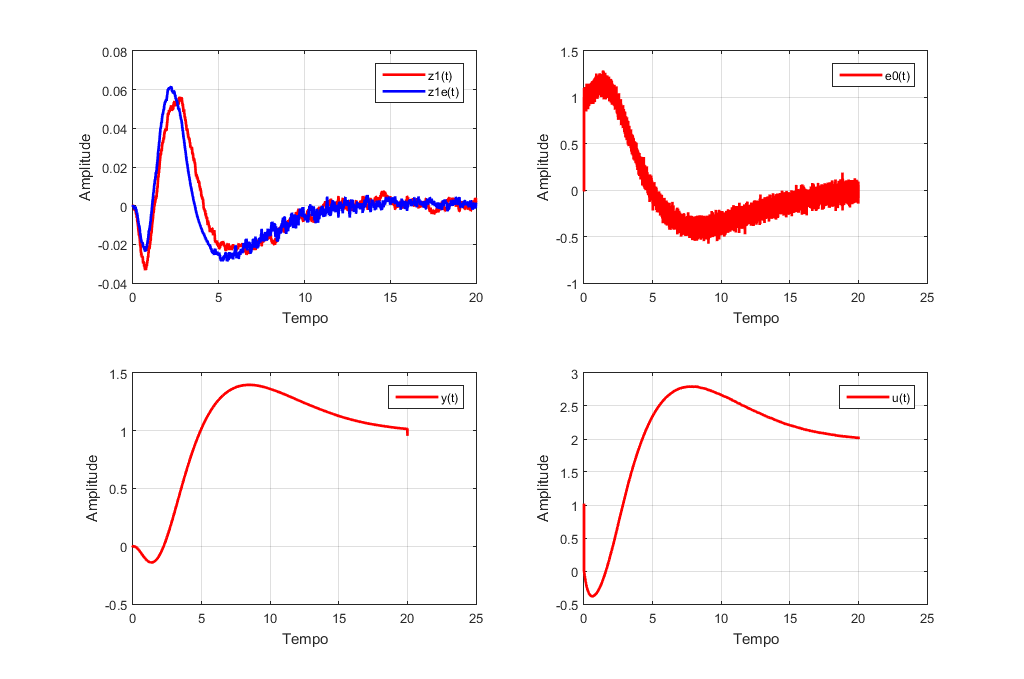
\includegraphics[width = \linewidth]{./pics/APPC_Correntropia_Ruido_Gaussiano.png}
\caption{APPC-MCC num ambiente de simulação  com ruído gaussiano aditivo de média 0 e variância 0.05, similarmente ao APPC-LSE, observamos a convergência de $\epsilon$ para 0}
\end{figure}

\subsection{Com Ruído Uniforme, $n_0 = 0.1$ para $0.5<x<0.5$}


Os resultados se encontram nas Figuras 7 e 8, para o LSE e MCC respectivamente.

\begin{figure}[htpb!]
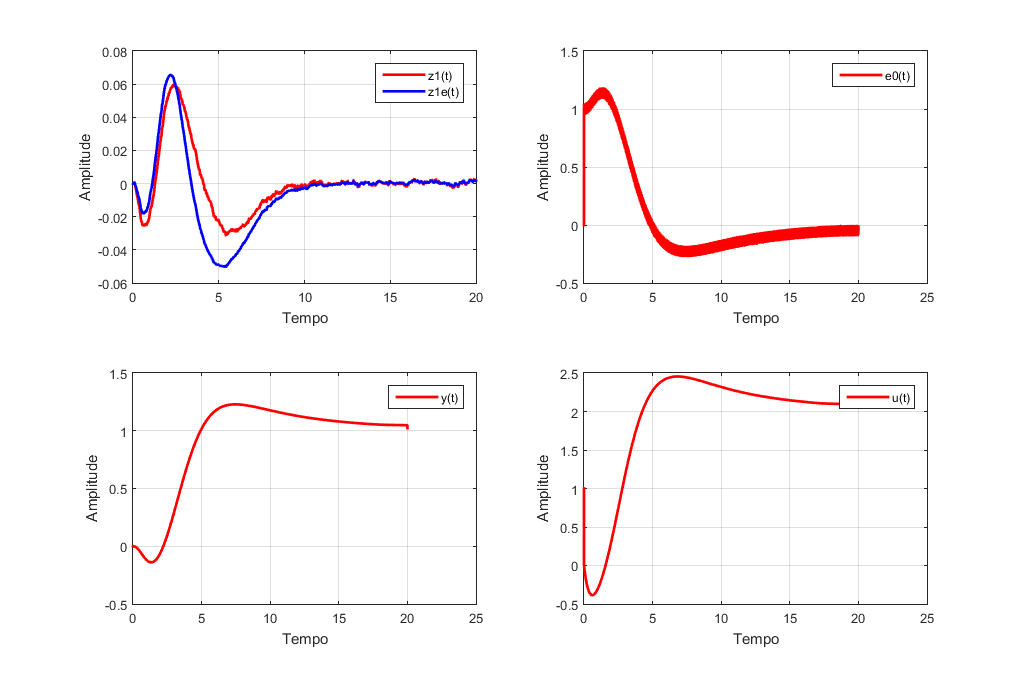
\includegraphics[width = \linewidth]{./pics/APPC_MSE_Ruido_Uniforme.png}
\caption{APPC-LSE num ambiente de simulação com ruído de distribuição uniforme aditivo, observa-se a convergência de $\hat{z}$ para $z$ e portanto $\epsilon \rightarrow 0$ a medida que $t \rightarrow \infty$, como esperado }
\end{figure}

\begin{figure}[htpb!]
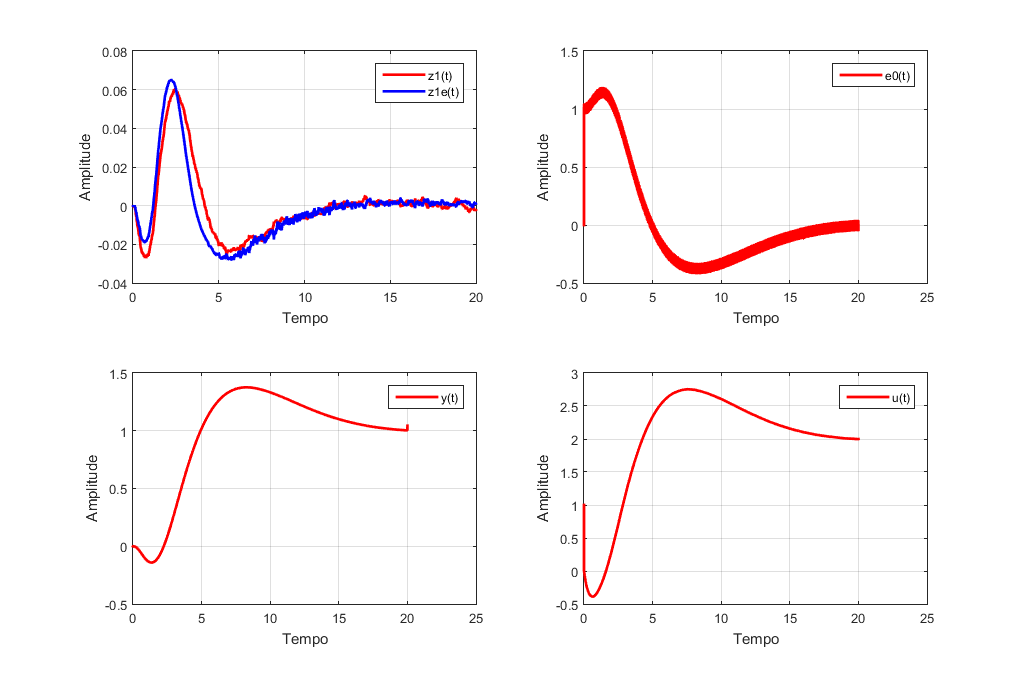
\includegraphics[width = \linewidth]{./pics/APPC_Correntropia_Ruido_Uniforme.png}
\caption{APPC-MCC num ambiente de simulação  com ruído de distribuição uniforme aditivo, similarmente ao APPC-LSE, observamos a convergência de $\epsilon$ para 0}
\end{figure}

\subsection{Com Ruído Impulsivo}

As simulações foram feitas com ruído de medição da variável $y(t)$ da saída da planta do tipo impulsivo com os seguintes valores:

\begin{equation}
\label{eq:Distribuição do ruído}
\displaystyle \eta_o(x) = \left\{
\begin{array}{rl}
       0 &\mbox{se $0.08<x<0.92$} \\
       2 &\mbox{se $x>0.92$}      \\
      -2 &\mbox{se $x<0.08$}      
\end{array}, \right.
\end{equation}

Onde x é uma variável aleatória com distribuição de probabilidade uniforme entre $0$ e $1$ e $n_o(x)$ é o ruído aditivo que contamina a medição de $y(t)$. Fizemos também simulações para ambos os sistemas no caso ideal sem ruído, que estão contidas nas figuras a seguir.\\


Os resultados se encontram nas Figuras 9 e 10, para o LSE e MCC respectivamente.

\begin{figure}[htpb!]
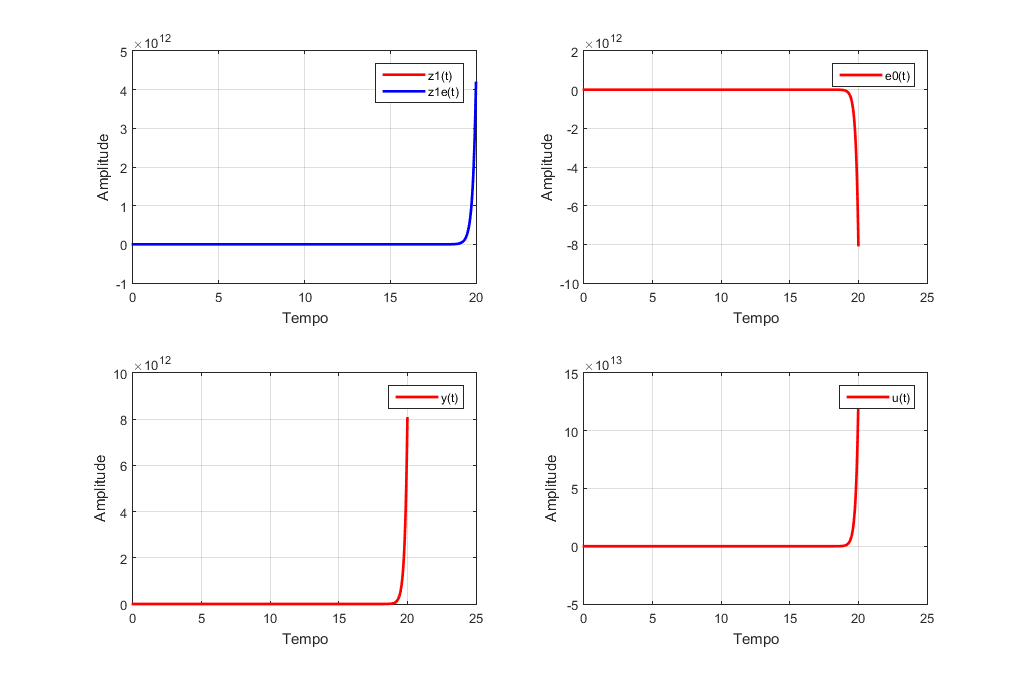
\includegraphics[width = \linewidth]{./pics/APPC_MSE_Ruido_Impulsivo.png}
\caption{APPC-LSE num ambiente de ruído impulsivo. O sinal de controle revela uma falha catastrófica no comportamento do controlador, que se dá devido a não-gaussianidade do ruído de medição}
\end{figure}

\begin{figure}[htpb!]
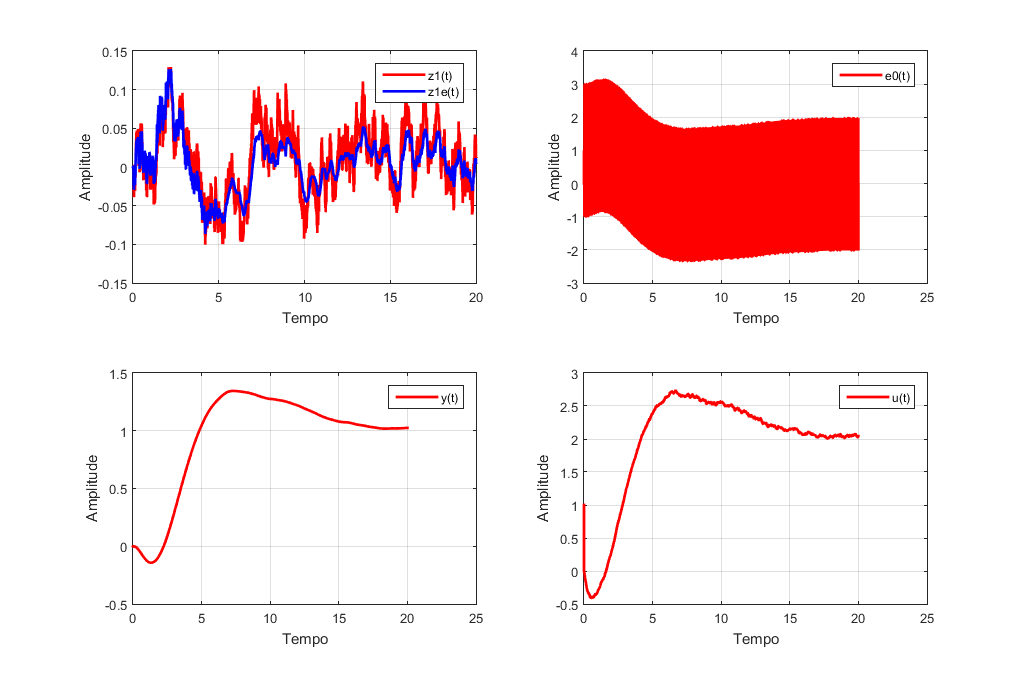
\includegraphics[width = \linewidth]{./pics/APPC_Correntropia_Ruido_Impulsivo.png}
\caption{APPC-MCC num ambiente de ruído impulsivo. O controlador proposto consegue corretamente rejeitar o ruído de medição impulsivo e fazer o controle desejado da planta}
\end{figure}


\pagebreak
\section{Conclusões}
~~~~       Como foi mostrado nas simulações o controlador proposto APPC-MCC possui robustez em relação ao ruído impulsivo e desempenho comparável ao APPC-LSE na ausência de ruído de medição. Isto não é surpreendente pois a Correntropia do erro representa uma norma híbrida, L2 para erros pequenos, L1 para uma determinada região e L0 para erros muito grandes, de forma que seu desempenho é comparável ao de um critério L2 na ausência de ruído de medição, porém é capaz de rejeitar dados muito discrepantes ("outliers") na medição dependendo da seleção do tamanho do kernel. Adicionalmente notamos que o custo computacional é de mesma magnitude entre os dois métodos.\\


~~~~       Em trabalhos futuros outros tipos de ruído não-gaussiano podem ser introduzidos na medição da saída da
planta. Gostaríamos também de investigar o Controle Adaptativo Indireto por Modelo de Referência para Grau Relativo qualquer da planta usando o estimador de parâmetros com critério MCC.\\


\section*{Agradecimentos}
%Agradeço a ~~, ~~, e ~~. E aos colegas ~~ e ~~.

%Para domingo: Corrigir Figuras.., Buscar referências, Tentar novamente achar artigo "recursive least square with stochastic gradient", testar MCC usando estimador de \hat{V} em janela de N amostras

% BIBLIOGRAFIA
\bibliography{bib-controleadaptativo}
\end{document}
